\chapter{KLASIČNI PRISTUP UPRAVLJANJU}
\label{ch:klasicni}

Klasični pristup rješava zadatak otvaranja vrata i prolaska kroz njih kao slijed jasno
odvojenih faza, od kojih svaka koristi eksplicitno poznavanje geometrije zadatka: poze kvake
iz percepcije, poznatog oblika prihvatnice i, za zakretna vrata, geometrijski izračunate osi
šarke. To je bitna razlika prema pristupu iz poglavlja \ref{ch:rl}.

\section{Struktura zadatka}
\label{sec:faze}

Zadatak je organiziran u četiri faze: prilaz, hvat, otvaranje i prolazak. Tip vrata robot prepoznaje
sam, iz geometrije kvake, tijekom faze hvata (potpoglavlje \ref{sec:prilaz}).
Ta odluka određuje koja se grana faze otvaranja pokreće.
Prolazak kroz vrata izveden je za oba tipa, uz razliku u načinu vođenja opisanu u
potpoglavlju \ref{sec:prolazak}. Slijed je prikazan na slici \ref{fig:faze}.

\begin{figure}[H]
      \centering
      \resizebox{\textwidth}{!}{
            \begin{tikzpicture}[
                        font       = \small,
                        box/.style = {draw, rounded corners=2pt, align=center, inner sep=5pt,
                                    minimum height=10mm, minimum width=26mm, fill=black!5},
                        term/.style= {box, fill=black!12},
                        ar/.style  = {-{Stealth[length=2mm]}, semithick}
                  ]
                  \node[term] (start) at (0,0)     {start};
                  \node[box]  (prilaz) at (3.3,0)  {prilaz};
                  \node[box]  (hvat)   at (6.6,0)  {hvat};
                  \node[box]  (slide)  at (10.4,0.9)  {\texttt{open\_sliding}\\[-1pt]\scriptsize klizna vrata};
                  \node[box]  (arc)    at (10.4,-0.9) {\texttt{open\_revolute}\\[-1pt]\scriptsize zakretna vrata};
                  \node[box]  (pass)   at (14.4,0)  {\texttt{pass\_through\_door}};
                  \node[term] (end)    at (18.0,0) {kraj};

                  \draw[ar] (start) -- (prilaz);
                  \draw[ar] (prilaz) -- (hvat);
                  \draw[ar] (hvat.north) |- (slide.west);
                  \draw[ar] (hvat.south) |- (arc.west);
                  \draw[ar] (slide.east) -| (pass.north);
                  \draw[ar] (arc.east)   -| (pass.south);
                  \draw[ar] (pass) -- (end);
            \end{tikzpicture}
      }
      \caption{Slijed faza klasičnog pristupa}
      \label{fig:faze}
\end{figure}

\section{Faza prilaza i hvata}
\label{sec:prilaz}

\subsection{Poravnanje platforme}
\label{sec:poravnanje}

Platforma se dovodi na određenu udaljenost od vrata (potpoglavlje \ref{sec:perception-iface})
regulacijom položaja prema velikoj oznaci na sredini vrata. Cilj regulacije nije samo
udaljenost, nego potpuna poza u ravnini, tj. bočni i uzdužni položaj te zakret, sve do zadanih
tolerancija.

Ciljna točka i ciljni zakret određeni su duž normale vrata, izvedene iz orijentacije
oznake, a ne samo iz smjera pogleda prema njoj. Regulacija koja nastoji držati oznaku na
sredini pogleda kamere ne jamči da će platforma stati okomito na vrata. Ako orijentacija
oznake iz nekog razloga nije dostupna, sustav se vraća na regulaciju smjera pogleda, čime
se izbjegava da robot potpuno stane, po cijenu manje pouzdanog poravnanja.

\subsection{Prepoznavanje tipa kvake}
\label{sec:tip-kvake}

Kad je platforma na ciljanoj udaljenosti, sustav sam prepoznaje tip vrata iz geometrije kvake,
umjesto da mu se tip zadaje pri pokretanju. Kvaka nosi dvije male oznake (potpoglavlje
\ref{sec:raspored-oznaka}); vektor između njihovih položaja jednoznačno razlikuje tipove, jer je
kod zakretnih vrata poluga kvake vodoravna, a kod kliznih šipka okomita. Kriterij je jednostavan
prag na okomitoj komponenti tog vektora: ako ona prelazi 70\,\% duljine vektora, kvaka je
okomita i vrata su klizna, inače su zakretna. Prepoznati tip određuje koja se od dviju unaprijed
zadanih početnih poza manipulatora koristi u nastavku, a poslije i koja se grana faze otvaranja
pokreće (potpoglavlje \ref{sec:otvaranje}).

\subsection{Hvat}
\label{sec:hvat-postupak}

\begin{enumerate}
      \item \textbf{Ponovno čitanje poze.} Na početnoj udaljenosti kvaka je izvan dosega
            manipulatora pri nepomičnoj platformi, pa se platforma nakon prvog očitanja poze
            dodatno primakne. Poza kvake se pritom ne prati kontinuirano, nego se rekonstruira iz
            njezina nepromjenjivog odnosa prema velikoj oznaci, koja ostaje u vidnom polju
            tijekom cijelog primicanja.
      \item \textbf{Prilaz.} Manipulator se dovodi u pozu prilaska ispred kvake te se zatim
            približava do konačne poze hvata.
      \item \textbf{Bočna korekcija.} Parovi prstiju prihvatnice ne gibaju se savršeno
            simetrično, pa se hvat sam od sebe ne centrira nad predmetom. Umjesto da se ta
            asimetrija ukloni, ona se mjeri: uspoređuju se položaji suprotnih prstiju tijekom
            zatvaranja, a iz njihove razlike izračunava se bočna korekcija kojom se prihvatnica
            poravna nad kvakom prije konačnog zatvaranja.
      \item \textbf{Korekcija dubine (engl. \textit{hill-climbing}).} Prihvatnica postupno
            prilagođava svoju dubinu duž osi prilaza kako bi šipka kvake u potpunosti sjela u
            utor prstiju. Pri svakom pokušaju prsti se zatvaraju do zaustavljanja i mjeri se
            ostvareni stupanj zatvorenosti; ako se mjera pogorša u odnosu na prethodni pokušaj,
            algoritam mijenja smjer pomaka i vraća se na dotad najbolju poziciju, sve dok se ne
            postigne željena dubina hvata ili se ne obavi najveći dopušteni broj pokušaja.
\end{enumerate}

\subsection{Sidrenje cilja na oznaku}
\label{sec:sidrenje}

Neposredno nakon potvrđenog hvata mjeri se i pohranjuje fiksan prostorni odnos između vrha
alata i velike oznake, tj. pomak i zakret koji vrijede u tom trenutku. Taj se odnos u nastavku
zadatka koristi za određivanje cilja gibanja: umjesto da se cilj izvodi iz posljednje poznate
poze vrha alata, on se u svakom koraku iznova računa iz trenutne poze oznake i pohranjenog
odnosa. Razlika je bitna kad kvaka unutar hvata blago klizne, što se pokazalo mjerljivim pri
otvaranju zakretnih vrata (potpoglavlje \ref{sec:otvaranje-zakretna}): bez sidrenja na oznaku,
cilj bi klizio zajedno s kvakom, klizanje se ne bi moglo ni izmjeriti, a manipulator nikad ne bi
dobio naredbu da nadoknadi razliku. Isti se mehanizam koristi i za neovisno mjerenje samog
klizanja, kao razlike između očekivane i stvarno postignute poze vrha alata.

\section{Faza otvaranja}
\label{sec:otvaranje}

Nakon uspješnog hvata, kreće faza otvaranja vrata.

Nakon uspješnog hvata, manipulator do kraja faze otvaranja ostaje u dostignutoj konfiguraciji
ili joj se vraća između malih koraka gibanja, a cjelokupno napredovanje izvodi platforma, uz
iznimku opisanu u potpoglavlju \ref{sec:otvaranje-zakretna}. Ta je odluka namjerna i vezana je
uz procjenu sile opisanu u poglavlju \ref{ch:procjena}: postupak umjeravanja procjenitelja
momenta vrijedi za konfiguraciju u kojoj je proveden (potpoglavlje \ref{sec:wrench-svojstva}),
pa svaki veći pomak manipulatora tu procjenu čini nevaljanom, osim ako se umjeravanje ponovi.

\subsection{Klizna vrata}
\label{sec:otvaranje-klizna}

Kod kliznih vrata smjer gibanja poznat je unaprijed --- vodoravna translacija duž zgloba
klizanja --- pa se platformi zadaje trapezni profil brzine u tom smjeru, s ubrzanjem,
ravnomjernom fazom i usporavanjem. Sam taj smjer izvodi se iz orijentacije
prihvatnice, i to iz njezine lokalne osi $x$, duž koje se prsti zatvaraju (potpoglavlje
\ref{sec:gripper}), projicirane na vodoravnu ravninu. Smjer se ne računa jednom na početku, nego se
osvježava u svakom koraku iz trenutne orijentacije prihvatnice. Kad bi ostao fiksan, a platforma
se u međuvremenu neznatno zakrenula, počela bi se stvarati komponenta sile koja stoji okomito na vrata
umjesto duž njih, a rasla bi s nakupljenim zakretom. Regulacija brzine prema izmjerenoj
sili namjerno nije korištena: sila uvijek naraste u trenutku kretanja platforme iz mirovanja, pa
bi svaki takav povratni regulator uveo zastajkivanje umjesto glatkog gibanja. Sila se koristi
isključivo kao sigurnosni prekid.

Hod kliznih vrata premašuje ono što platforma stigne prijeći unutar jednog trapeznog profila, pa
se vožnja prema potrebi ponavlja u više prolaza, bez ponovnog hvata. Prihvatnica drži
kvaku neprekidno, platforma se samo zaustavi na kraju jednog profila i ponovno krene s početka
sljedećeg. Napredak nakon svakog prolaza provjerava se iz percepcije, kao pomak velike oznake
izražen u nepomičnom okviru: poza oznake u koordinatnom sustavu platforme pretvara se u taj okvir
pomoću odometrije (potpoglavlje \ref{sec:odometrija}). Odstupanje tako dobivenog pomaka od
stvarnog stanja zgloba vrata iznosi 44 mm, odnosno 4,6 \%.

\subsection{Zakretna vrata}
\label{sec:otvaranje-zakretna}

Kod zakretnih vrata gibanje platforme nije jednostavna translacija, pa način na koji je
otvaranje ostvareno bitno odstupa od kliznih vrata: umjesto da precizno praćenje luka izvodi
platforma, tu je zadaću preuzeo manipulator, dok platforma ima samo pomoćnu ulogu.

Otvaranje se izvodi u dvije uzastopne faze: guranjem, u kojem robot kvaku vodi po luku, i
završnim zakretom platforme, kojim se vrata doguravaju do konačnog kuta.

Tijekom guranja platforma se giba po smjeru tangente luka kvake, a manipulator u svakom koraku
zakreće vrh alata za mali kut duž procijenjene kružnice, inverznom kinematikom. Precizno vođenje
po luku time je prepušteno manipulatoru, a platformi ostaje gibanje po pravcu. Cilj se pritom
sidri na oznaku, na način opisan u potpoglavlju \ref{sec:sidrenje}, čime se u svakom koraku
nadovezuje na stvarno postignuto stanje kvake, a ne na vlastitu prethodnu naredbu.

Izbor smjera tangente za gibanje baze počiva na činjenici da se sila kojom baza gura prenosi kroz
krutu ruku na kvaku. Ako ta sila ima komponentu duž kvake, ta komponenta izvlači prihvatnicu s
kvake i hvat klizi.

Korak manipulatora nije fiksan, nego razmjeran trajanju prethodnog ciklusa upravljanja, uz gornju
granicu. Razlog je taj što platforma vozi neprekidno, a trajanje ciklusa određuje planiranje
gibanja i kreće se između 0,4 i 2,1 s; uz fiksni korak manipulator bi u duljem ciklusu zaostao za
platformom.

Mjerenja i sigurnosni prekidi ne izvode se u glavnoj petlji, nego u zasebnoj niti na 20 Hz. Kako
ciklus glavne petlje traje i do dvije sekunde, a platforma za to vrijeme vozi i vrata se otvore
15 do 18\textdegree{}, prag bi se inače uvijek prekoračio prije nego bi ga sustav primijetio. Ta
nit ujedno vodi regulator platforme i sama je zaustavlja čim uvjet prekida okine.

Budući da vrh alata inverznom kinematikom vodi MoveIt, prije početka povlačenja iz njegove
planerske scene uklanjaju se kolizijski objekti vrata i zidova (potpoglavlje \ref{sec:vrata}).
U suprotnom bi planer odbijao upravo ono gibanje koje je namjerno usmjereno prema kvaki i
kroz prostor koji zid inače zatvara. Kolizijski objekti zida u planersku scenu ne ulaze kao dva
unaprijed poznata tijela, nego se sastavljaju iz skena lidara, pa njihov broj nije unaprijed
određen. Kad su vrata zatvorena, krilo i oba zida optički čine jednu neprekinutu plohu, dok se
otvaranjem krilo odmakne i pojave se dva razdvojena segmenta.

Za razliku od procjene ograničenja iz poglavlja \ref{ch:procjena}, os šarke se ovdje ne
procjenjuje iz gibanja, nego se izravno izračunava iz geometrije poznate percepciji, i to iz
jednog, fiksnog vektora izraženog u koordinatnom sustavu same oznake. Neka je $\bm{p}_{\mathrm{tag}}$
položaj velike oznake, a $\bm{R}(\bm{q}_{\mathrm{tag}})$ matrica rotacije koja opisuje njezinu
orijentaciju. Os šarke procjenjuje se kao

\begin{equation}
      \bm{c} = \bm{p}_{\mathrm{tag}} + \bm{R}(\bm{q}_{\mathrm{tag}})\, \bm{v}_{\mathrm{hinge}} ,
      \qquad
      \bm{v}_{\mathrm{hinge}} = \begin{pmatrix} 0 \\[2pt] -L/2 \\[2pt] -\delta \end{pmatrix} ,
      \label{eq:axis}
\end{equation}

gdje je $\bm{c}$ procijenjeni položaj osi šarke. Računa se kao položaj velike oznake, pomaknut vektorom
$\bm{v}_{\mathrm{hinge}}$ koji je prethodno zaokrenut u svjetski koordinatni sustav istom
rotacijom kao i sama oznaka. Druga i treća komponenta tog vektora izražene su u lokalnim
osima oznake: $L$ je širina krila (tablica \ref{tab:vrata}), a $\delta = 21\text{ mm}$ odmak
oznake od središnje ravnine debljine krila. Slika \ref{fig:os-sarke} prikazuje konstrukciju u tlocrtu.

Vektor $\bm{v}_{\mathrm{hinge}}$ ima jednostavno geometrijsko značenje: oznaka je
postavljena točno na sredinu krila, pa je udaljenost do osi šarke, mjerena duž krila, jednaka
točno polovici njegove širine. Krilo je debelo 40 mm, a os šarke, kao i kod stvarnih vrata,
prolazi kroz sredinu te debljine, ne kroz plohu na kojoj je oznaka zalijepljena. Time nastaje
razmak od 20 mm (polovica debljine krila) kojemu se pridodaje i sitan odmak same naljepnice od plohe od
svega 1 mm, pa je ukupni $\delta$ 21 mm.

\begin{figure}[H]
      \centering
      \begin{tikzpicture}[
                  font    = \small,
                  pt/.style   = {circle, fill=black, inner sep=1.3pt},
                  leaf/.style = {very thick},
                  vec/.style  = {-{Stealth[length=2mm]}, semithick},
                  dvec/.style = {-{Stealth[length=2mm]}, densely dashed, semithick, gray!70!black}
            ]
            % os y (vodoravno na papiru) = duz krila; os x (okomito, "gore") = normala vrata
            \coordinate (hinge) at (0,0);
            \coordinate (foot)  at (4.25,0);
            \coordinate (tag)   at (4.25,1.3);
            \coordinate (edge)  at (8.5,0);

            \draw[leaf] (hinge) -- (edge);
            \node[pt] at (hinge) {}; \node[below=2pt] at (hinge) {$\bm{c}$ (šarka)};
            \node[pt] at (edge)  {}; \node[below=2pt] at (edge)  {slobodni rub};
            \node[pt] at (tag)   {}; \node[above=2pt] at (tag)   {$\bm{p}_{\mathrm{tag}}$};

            % lokalne osi oznake - iznad tocke oznake, odvojeno od konstrukcije ispod
            \draw[dvec] (tag) -- ++(0,0.9) node[above] {\scriptsize lokalna $z$};
            \draw[dvec] (tag) -- ++(-1.3,0) node[left] {\scriptsize lokalna $y$};

            % korak 1: ispravak odmaka delta (tag -> foot, okomito dolje na ravninu vrata)
            \draw[vec] (tag) -- (foot) node[midway, right] {\scriptsize $-\delta$};

            % korak 2: pomak za L/2 duz krila (foot -> hinge)
            \draw[vec, thick] (foot) -- (hinge) node[midway, above] {\scriptsize $-L/2$};

            \draw[<->] (0,-0.9) -- node[fill=white,inner sep=1pt] {\scriptsize $L/2$} (4.25,-0.9);
            \draw[<->] (4.25,-0.9) -- node[fill=white,inner sep=1pt] {\scriptsize $L/2$} (8.5,-0.9);
      \end{tikzpicture}
      \caption{Konstrukcija procjene osi šarke iz poze i lokalnih osi velike oznake, tlocrt}
      \label{fig:os-sarke}
\end{figure}

Izraz \eqref{eq:axis} vrijedi iz jednog, trenutnog očitanja poze oznake, bez praćenja kuta vrata
kroz vrijeme: kako oznaka rotira zajedno s krilom oko prave, nepomične osi šarke, umnožak
$\bm{R}(\bm{q}_{\mathrm{tag}})\,\bm{v}_{\mathrm{hinge}}$ rotira s njom na jednak način, pa zbroj
u svakom trenutku ponovno pogađa istu točku u prostoru.

Oznaka se ipak koristi samo do hvata. Kako se vrata otvaraju, ona izlazi iz vidnog polja kamere,
pa se položaj osi šarke jednom utvrdi pri hvatu i dalje prati odometrijom (potpoglavlje
\ref{sec:odometrija}). To je moguće jer je os šarke nepomična u prostoru, pa je dovoljno pratiti
gibanje same platforme.

Iz istog razloga i kut otvorenosti vrata prati se posredno. Dok prihvatnica drži kvaku, smjer od
osi šarke prema vrhu alata ujedno je i smjer krila, pa se kut računa iz te dvije poze, i to u
nepomičnom okviru.

\subsection{Završni zakret platforme}
\label{sec:zavrsni-zakret}

Guranje se zaustavlja na 70\textdegree{}, iz razloga navedenog u potpoglavlju
\ref{sec:klasicni-limits}. Taj kut nije dovoljan za prolazak, pa slijedi druga faza, u kojoj
platforma zakreće oko točke na sredini vlastite prednje strane, za otprilike 20\textdegree{}.

Bitna je razlika u tome što manipulator tijekom tog zakreta miruje u dosegnutoj konfiguraciji, a
prihvatnica i dalje drži kvaku. Cijeli se sklop (platforma, manipulator i krilo) giba kao
jedno tijelo, pa hvat nije dodatno opterećen. Za kruženje oko točke $\bm{c}$ izražene u
koordinatnom sustavu platforme, naredba brzine slijedi iz uvjeta da ta točka miruje:

\begin{equation}
      v_x = \omega\, c_y , \qquad v_y = -\omega\, c_x , \qquad \omega_z = \omega .
      \label{eq:pivot}
\end{equation}

Time se vrata doguravaju do otprilike 100\textdegree{} pa krilo više ne strši u prolaz, a
robot može nesmetano proći.

\section{Prolazak kroz vrata}
\label{sec:prolazak}

Nakon otvaranja slijedi prolazak, izveden za oba tipa vrata. Robot se ovdje oslanja na lidar
(potpoglavlje \ref{sec:lidar}).

Otvor se iz skena traži u dva koraka. Najprije se postupkom konsenzusa slučajnog uzorka
(\textit{RANSAC}, engl. \textit{Random Sample Consensus}) među točkama skena traži najizraženiji pravac,
koji odgovara ravnini zidova, uz uvjet da mu je smjer pretežno poprečan u odnosu na robota.
Taj je uvjet nužan jer bez njega, kad je robot blizu vrata, gusto uzorkovano krilo postane
najizraženiji pravac i klasifikacija pada. Zatim se među točkama koje pripadaju zidu
traži praznina širine bliske poznatoj širini dovratnika. Na mirujućem robotu središte i
širina tako pronađenog otvora ostaju točni i precizni unutar otprilike jednog centimetra.
Pred zatvorenim vratima postupak ispravno ne pronalazi ništa.

Postupak prolaska ima sljedeće korake:

\begin{enumerate}
      \item \textbf{Otpuštanje i povlačenje.} Prihvatnica otvara prste, a manipulator se povlači
            unazad duž osi prilaza, kako se pri odlasku u pozu parkiranja ne bi sudario
            sa šipkom kvake.
      \item \textbf{Parkiranje ruke.} Manipulator odlazi u unaprijed zadanu pozu iznad baze kako
            ne bi zapeo za zidove ili vrata tijekom prolaska.
      \item \textbf{Odmicanje i ispravljanje} (samo zakretna vrata). Platforma se odmiče
            0,35 m unatrag i ispravlja okomito na ravninu zida, čime dobiva prostor za manevar
            pred otvorom.
      \item \textbf{Poravnanje.} Platforma se bočno pomiče, holonomnim gibanjem u poprečnom
            smjeru, dok se pronađeni otvor ne dovede pred robota.
      \item \textbf{Prolazak.} Platforma se giba naprijed kroz otvor.
\end{enumerate}

Kod kliznih vrata prolazak je pravocrtan i bez korekcije, jer se krilo povuklo u stranu, a
poravnanje je dovršeno prije nego vožnja počne. Kod zakretnih vrata krilo pri 100\textdegree{}
više ne strši u koridor, ali ono zna ometati detekciju, pa se robot ne uspije poravnati savršeno
okomito. Vožnja se ondje vodi odbojnim poljem. Svaka zapamćena točka prepreke unutar
zadanog dometa gura robota od sebe, jače što je bliže, a doprinosi se zbrajaju i usrednjuju.
Zbroj preko stotina točaka mijenja se glatko pa nema oscilacija tijekom prolaska.

Tri su pojedinosti nužne da to radi. Polje se računa u točki nešto ispred robota, a ne oko
njegova trenutnog položaja, jer se ondje doprinosi s lijeve i desne strane međusobno poništavaju
dok je robot između prepreka, pa reakcija dolazi prekasno; krilo uz to strši ispred robota, ne
bočno. Doprinosi se ograničavaju po uzdužnoj osi, jer inače udaljeni dijelovi zida nadglasaju
krilo i polje na većoj udaljenosti pokazuje u krivu stranu. Naposljetku, polje upravlja samo
zakretom, bez bočne komponente, jer translacija ima istu mrtvu zonu opisanu u potpoglavlju
\ref{sec:klasicni-limits}, pa bi naredba bila ili puna ili nikakva.

Lidar se nalazi na prednjoj strani platforme, pa robot pri samom prolasku izgubi iz vida i zid i
krilo upravo kad su mu najbliži. Zbog toga se sve viđene točke pamte u nepomičnom okviru, sažete
u rešetku ćelija od pet centimetara. Udaljenost do prepreke pritom se računa do ruba pravokutnika
platforme, a ne do njezina središta, i točke se ne odbacuju prema tome jesu li iza robota, primjerice
dovratnik uz lijevi bok robota, kojeg je prednji rub upravo prošao, i dalje je opasan za stražnji kut.

\section{Rezultati}
\label{sec:rezultati-klasicni}

Slike \ref{fig:faze-klasicni-zakretna} i \ref{fig:faze-klasicni-klizna} prikazuju karakteristične
trenutke izvođenja na oba tipa vrata. Slijed je isti za oba, uz razliku u fazi otvaranja,
gdje kod zakretnih vrata nakon guranja slijedi završni zakret platforme.

\begin{figure}[H]
      \centering
      \begin{subfigure}[b]{0.48\textwidth}
            \centering
            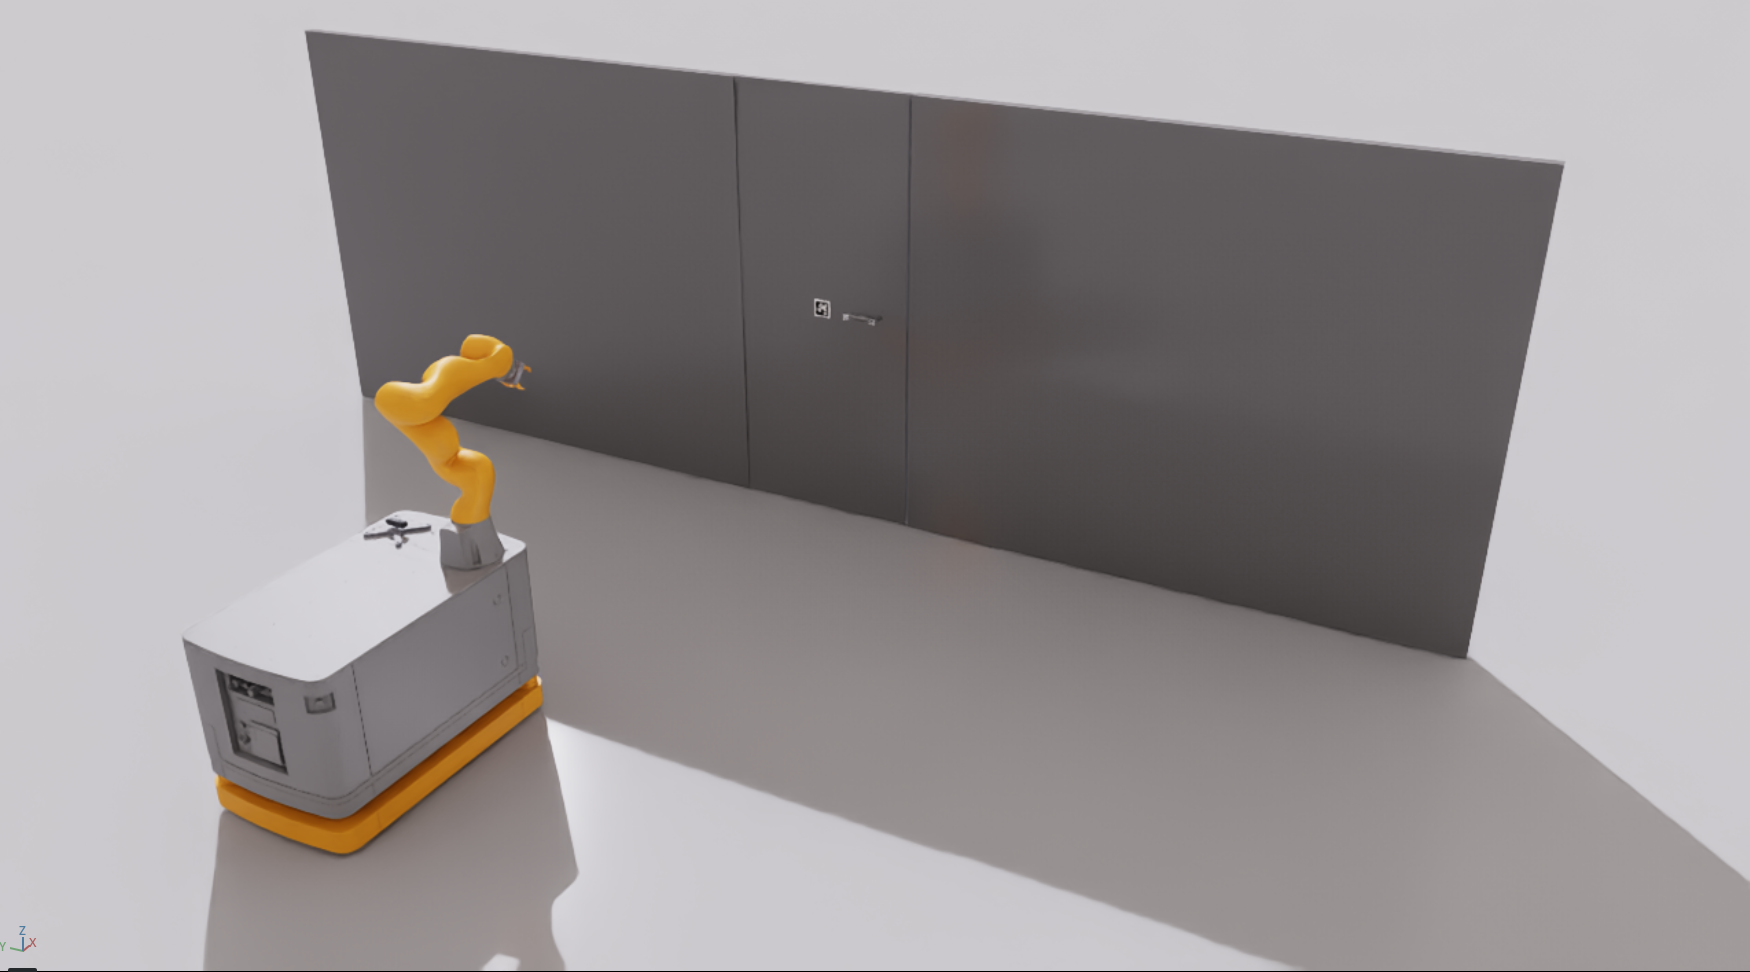
\includegraphics[width=\textwidth]{figures/kl_slike/kl_revolute_pocetak.png}
            \caption{početno stanje}
      \end{subfigure}
      \hfill
      \begin{subfigure}[b]{0.48\textwidth}
            \centering
            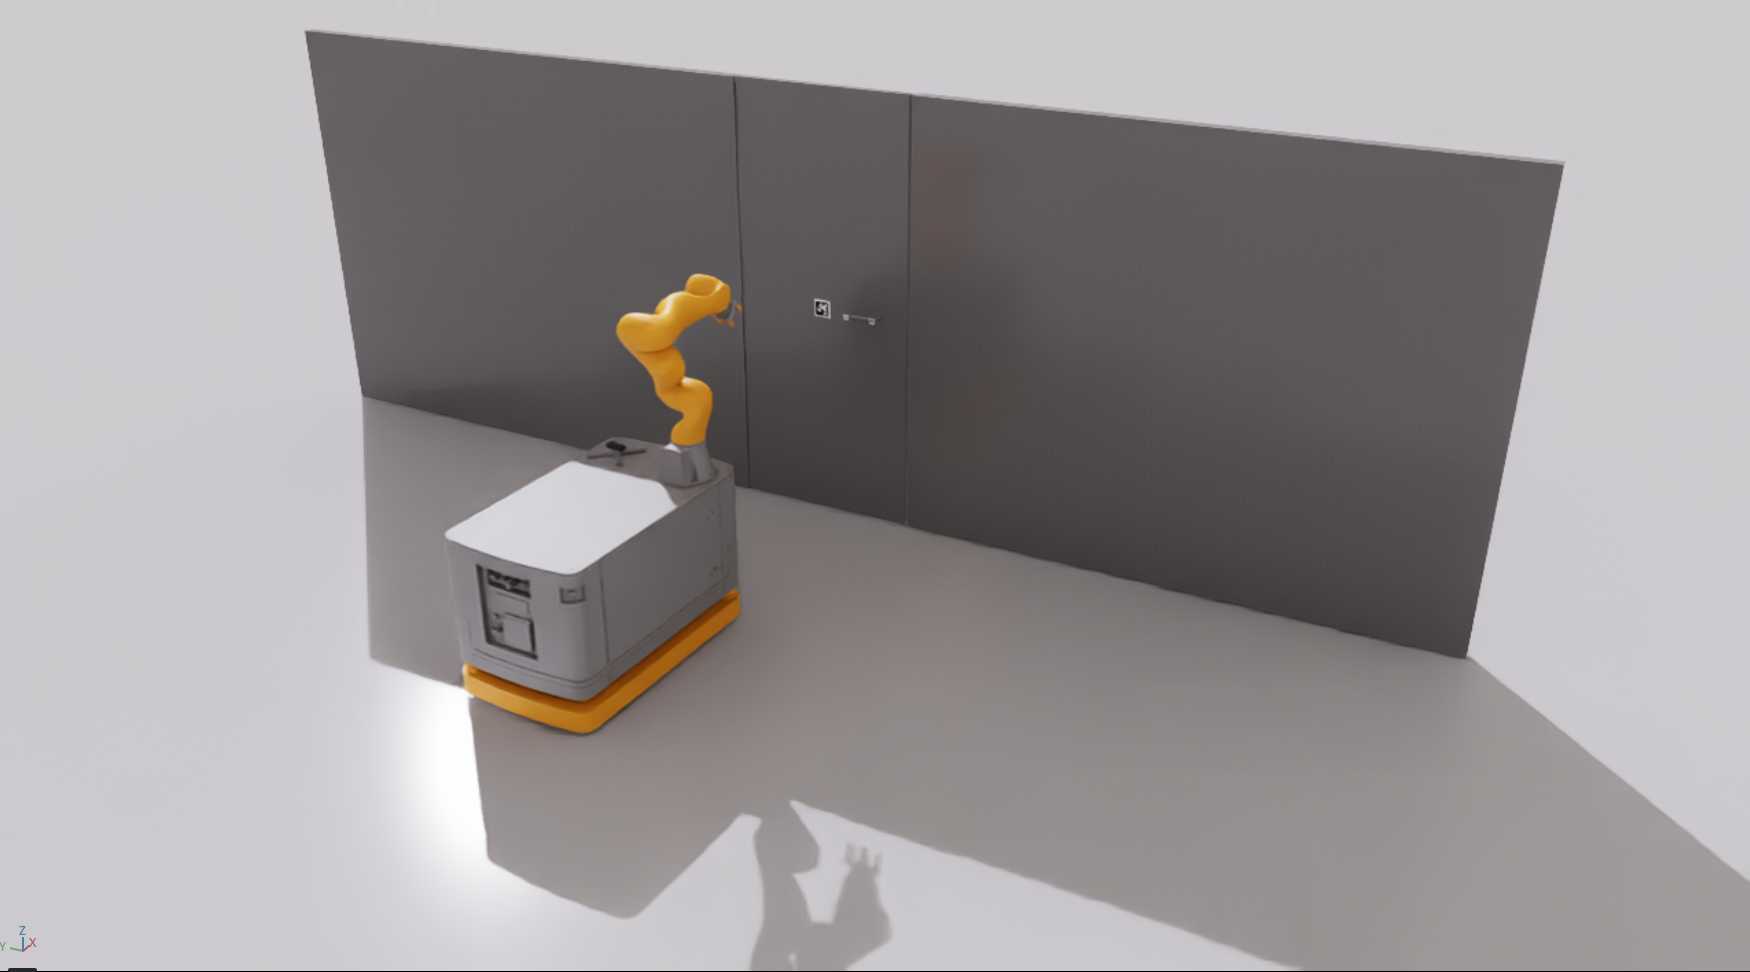
\includegraphics[width=\textwidth]{figures/kl_slike/kl_revolute_prilazak.png}
            \caption{prilazak vratima}
      \end{subfigure}

      \vspace{4pt}
      \begin{subfigure}[b]{0.48\textwidth}
            \centering
            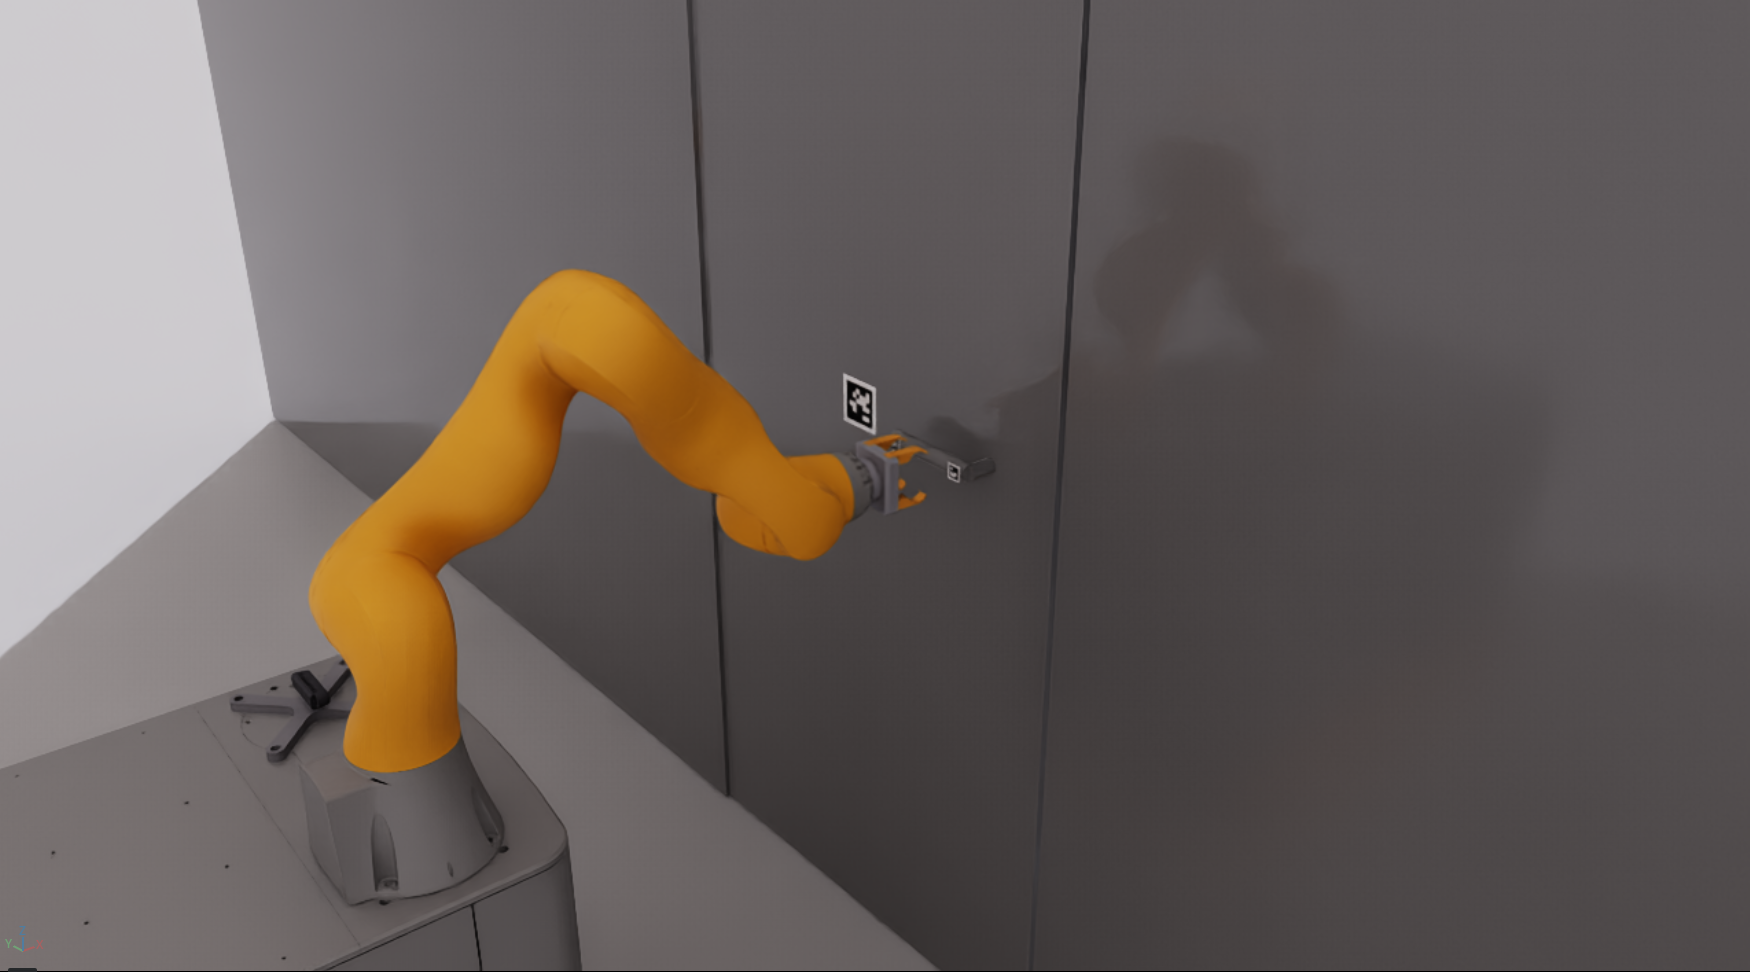
\includegraphics[width=\textwidth]{figures/kl_slike/kl_revolute_hvat.png}
            \caption{hvat kvake}
      \end{subfigure}
      \hfill
      \begin{subfigure}[b]{0.48\textwidth}
            \centering
            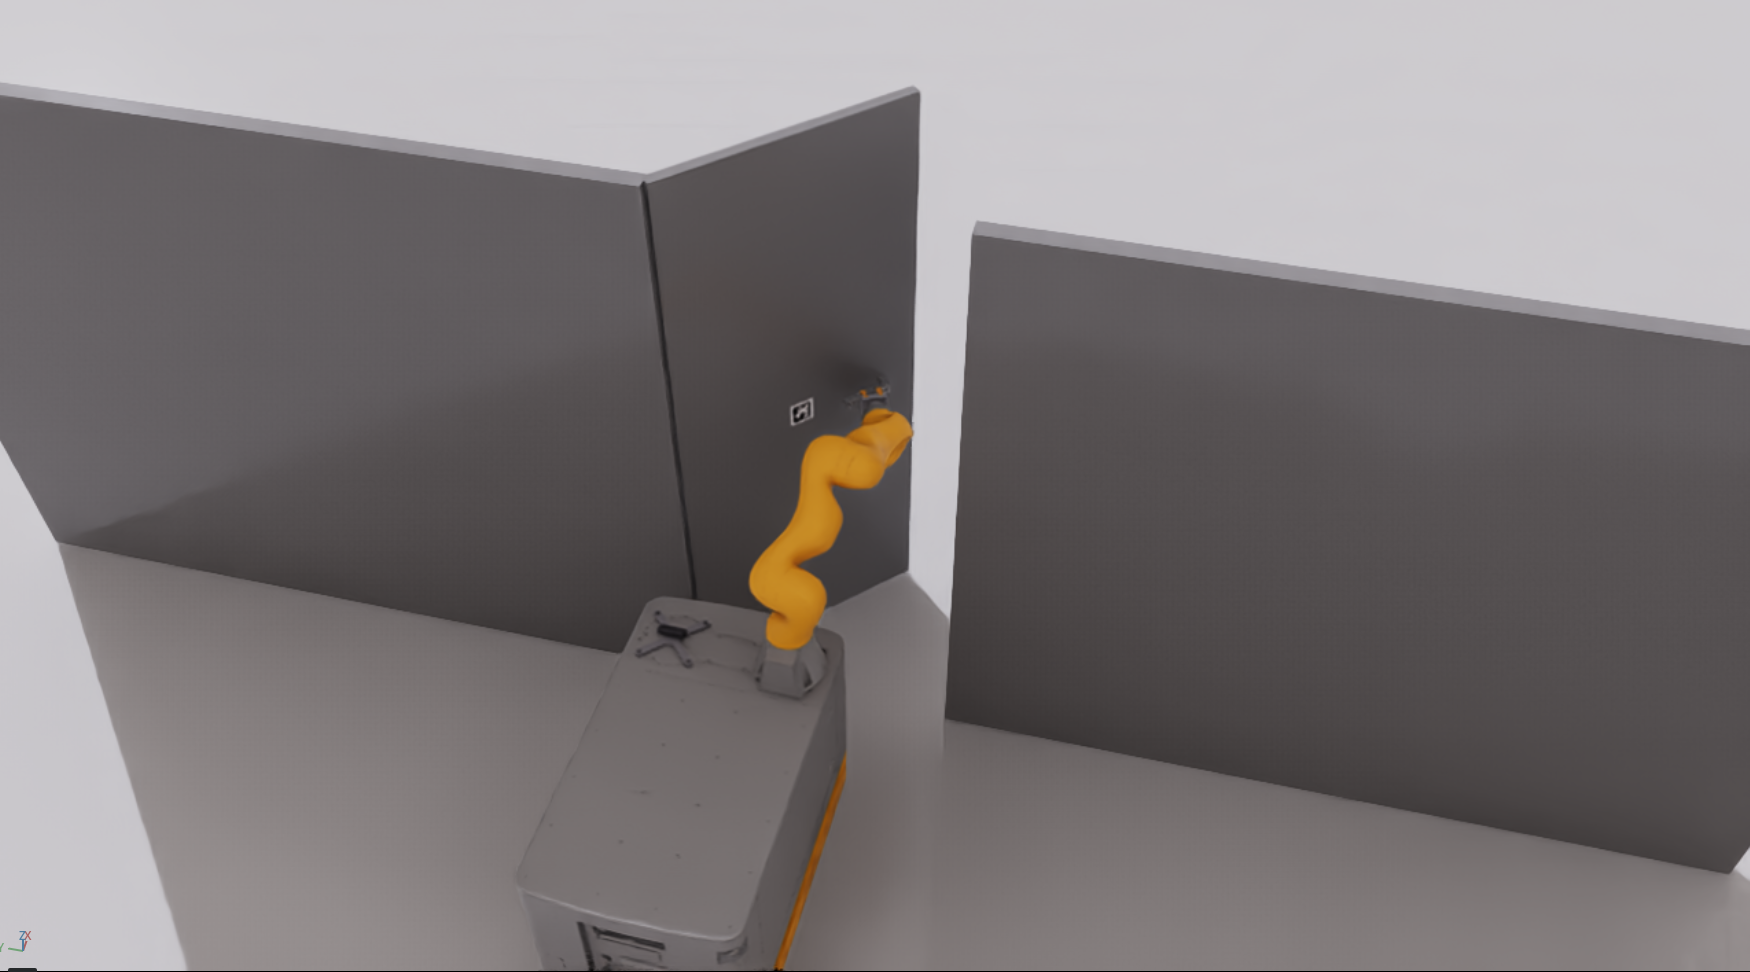
\includegraphics[width=\textwidth]{figures/kl_slike/kl_revolute_otvaranje.png}
            \caption{otvaranje}
      \end{subfigure}

      \vspace{4pt}
      \begin{subfigure}[b]{0.48\textwidth}
            \centering
            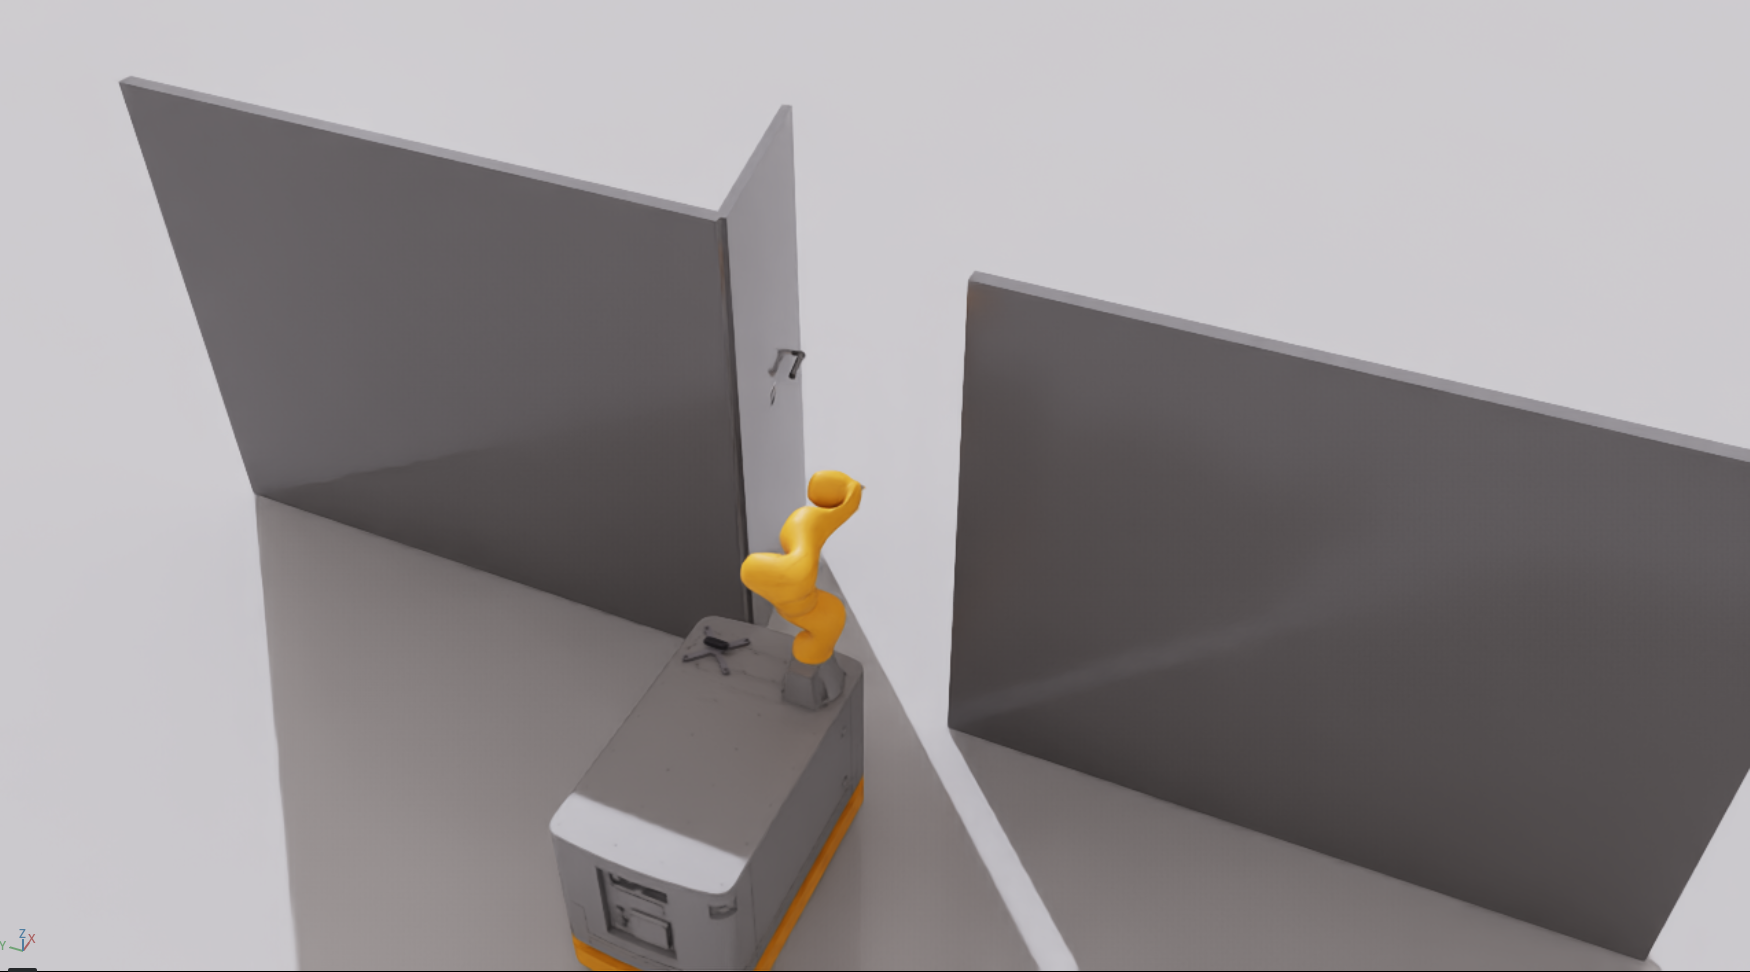
\includegraphics[width=\textwidth]{figures/kl_slike/kl_revolute_namjestanje.png}
            \caption{namještanje pred otvorom}
      \end{subfigure}
      \hfill
      \begin{subfigure}[b]{0.48\textwidth}
            \centering
            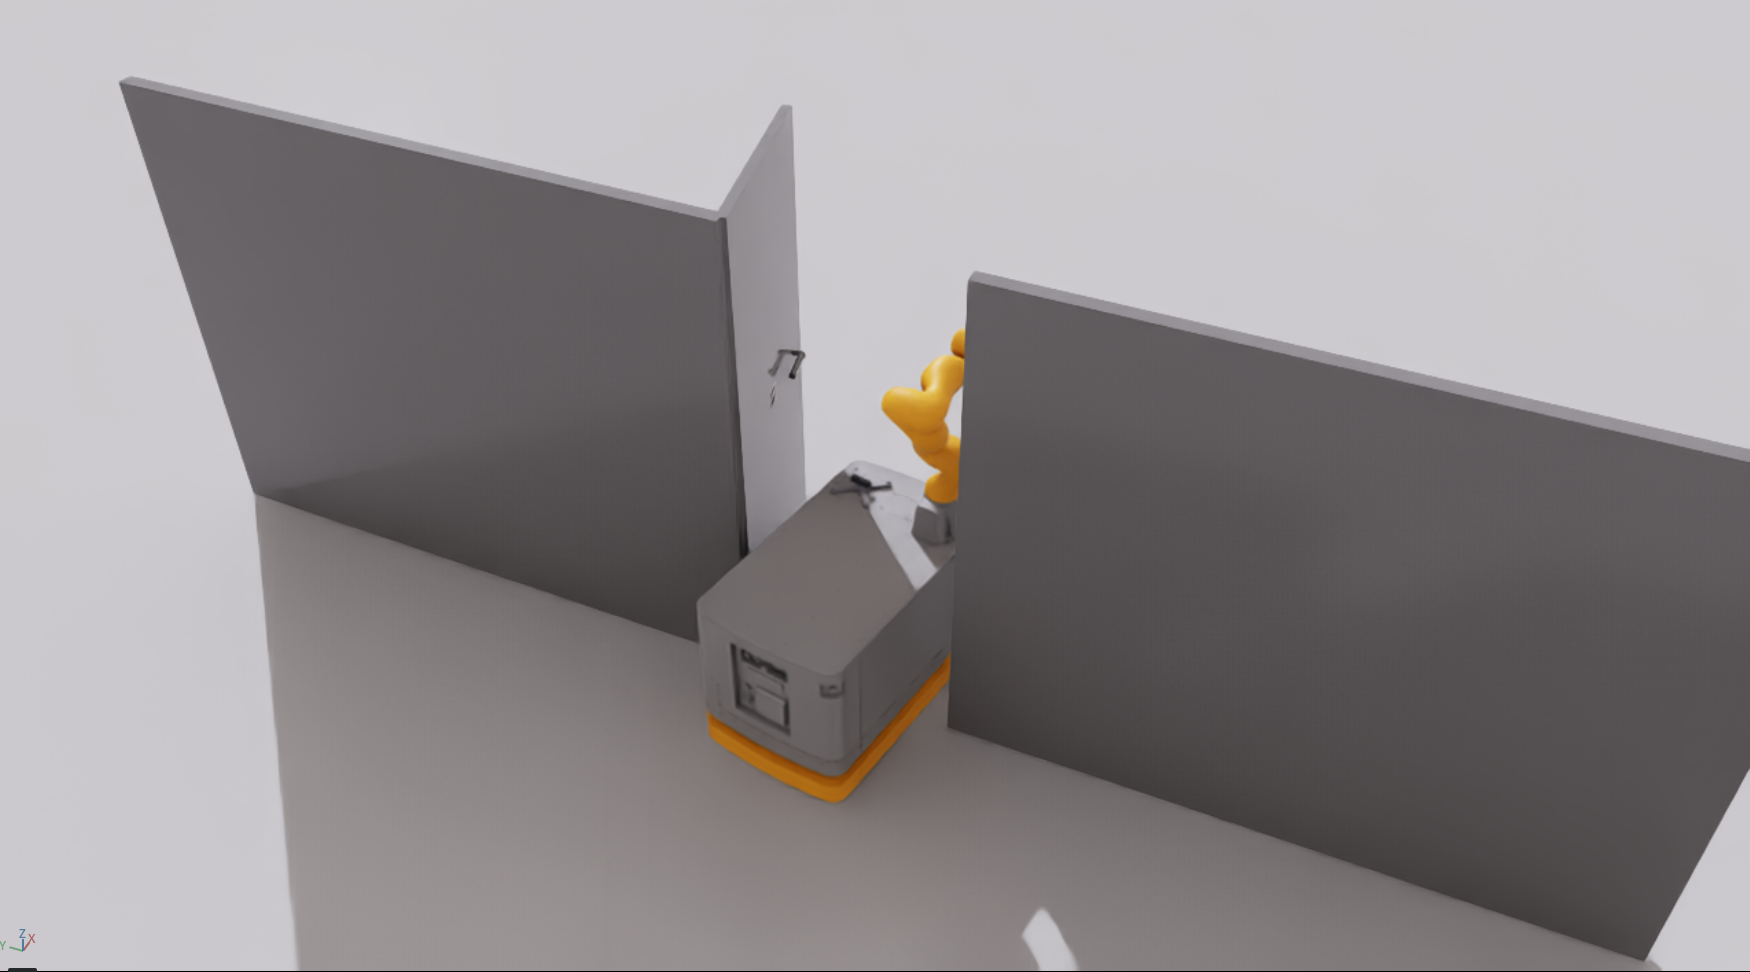
\includegraphics[width=\textwidth]{figures/kl_slike/kl_revolute_prolaz.png}
            \caption{prolazak kroz vrata}
      \end{subfigure}
      \caption{Faze izvođenja klasičnog pristupa na zakretnim vratima}
      \label{fig:faze-klasicni-zakretna}
\end{figure}

\begin{figure}[H]
      \centering
      \begin{subfigure}[b]{0.48\textwidth}
            \centering
            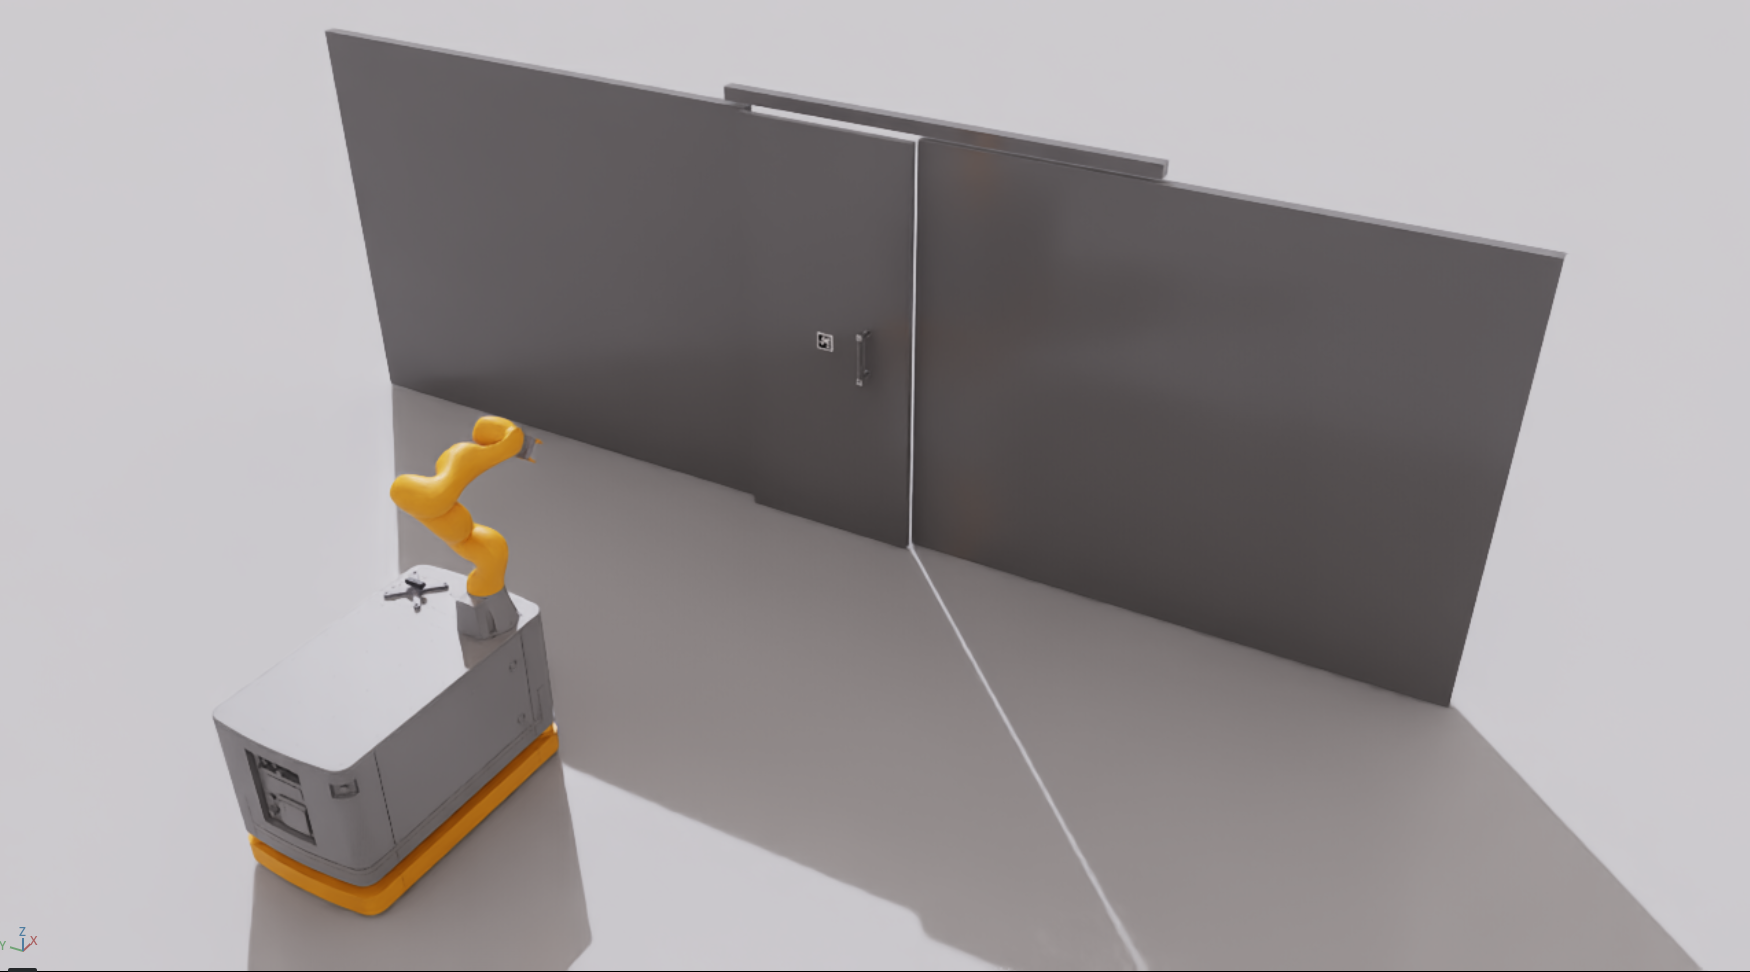
\includegraphics[width=\textwidth]{figures/kl_slike/kl_sliding_pocetak.png}
            \caption{početno stanje}
      \end{subfigure}
      \hfill
      \begin{subfigure}[b]{0.48\textwidth}
            \centering
            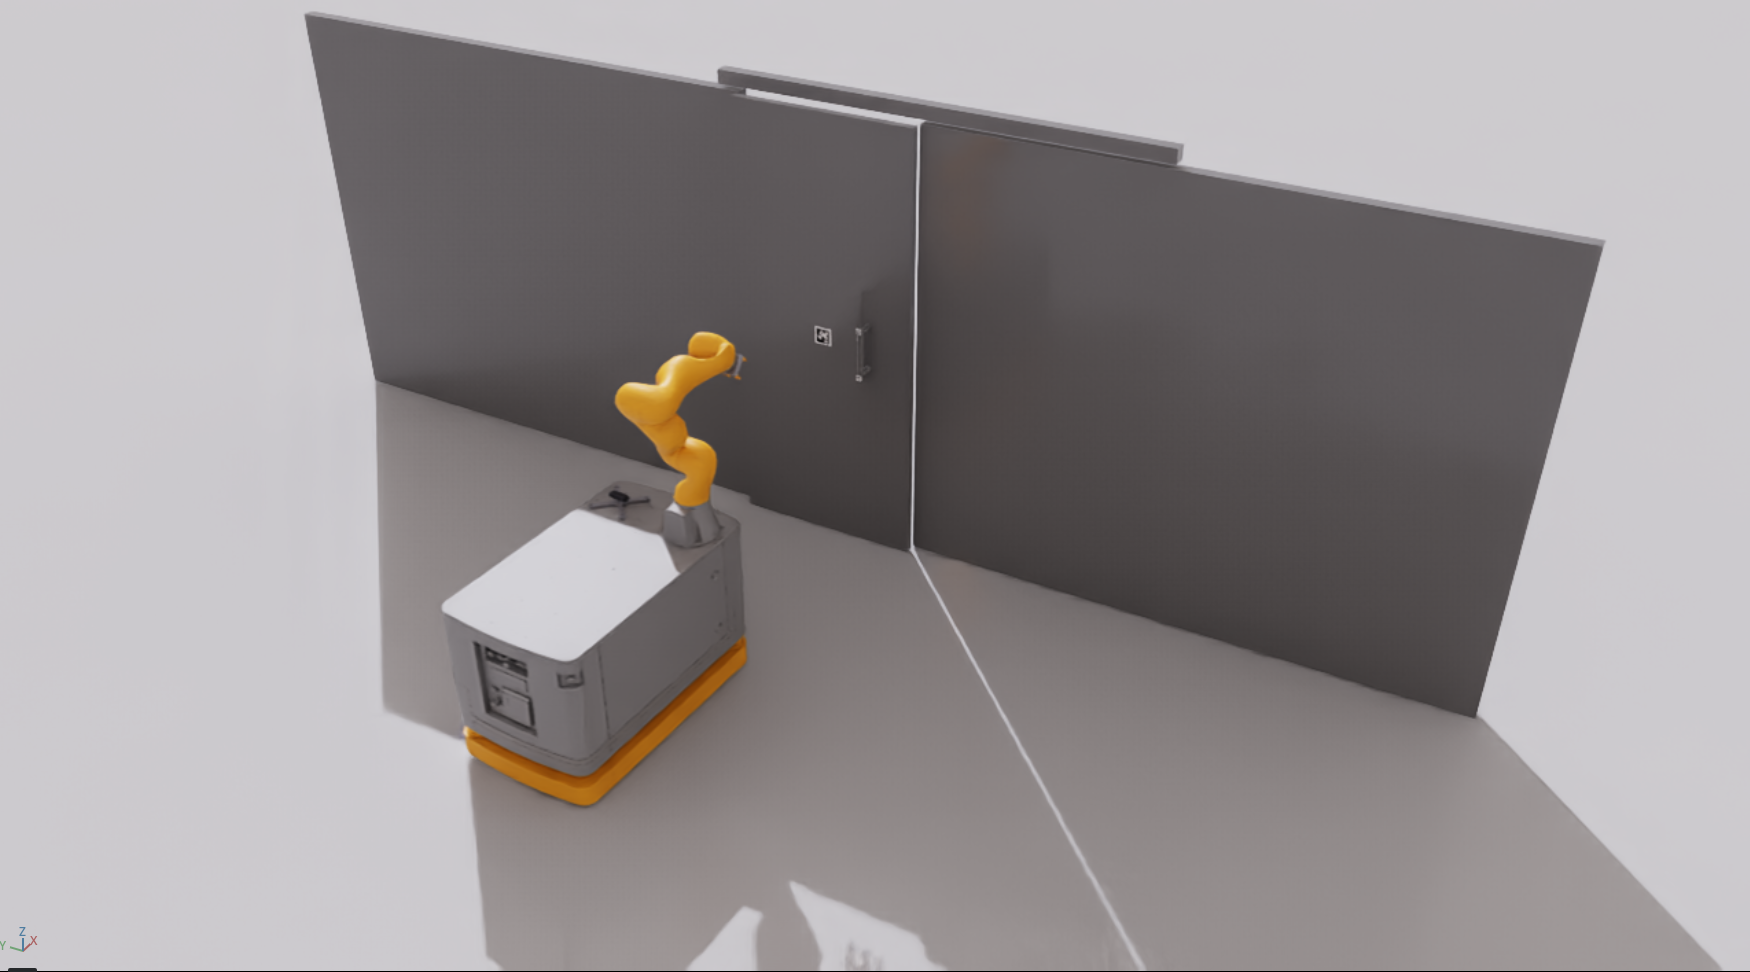
\includegraphics[width=\textwidth]{figures/kl_slike/kl_sliding_prilazak.png}
            \caption{prilazak vratima}
      \end{subfigure}

      \vspace{4pt}
      \begin{subfigure}[b]{0.48\textwidth}
            \centering
            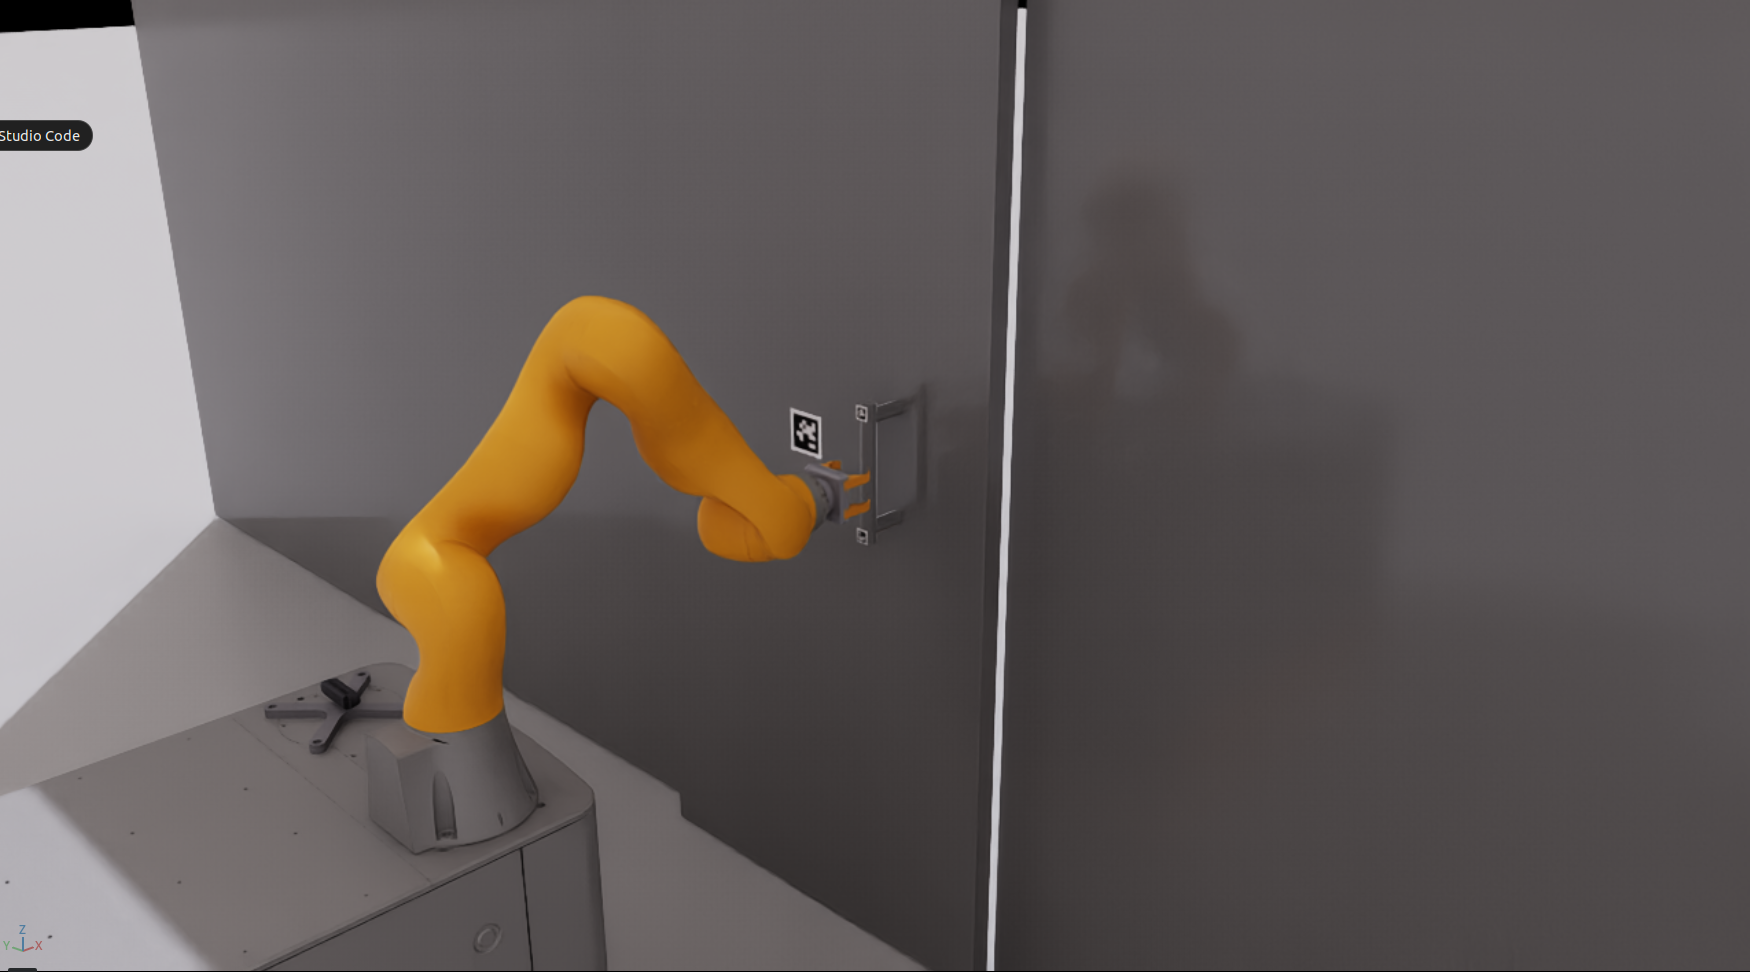
\includegraphics[width=\textwidth]{figures/kl_slike/kl_sliding_hvat.png}
            \caption{hvat kvake}
      \end{subfigure}
      \hfill
      \begin{subfigure}[b]{0.48\textwidth}
            \centering
            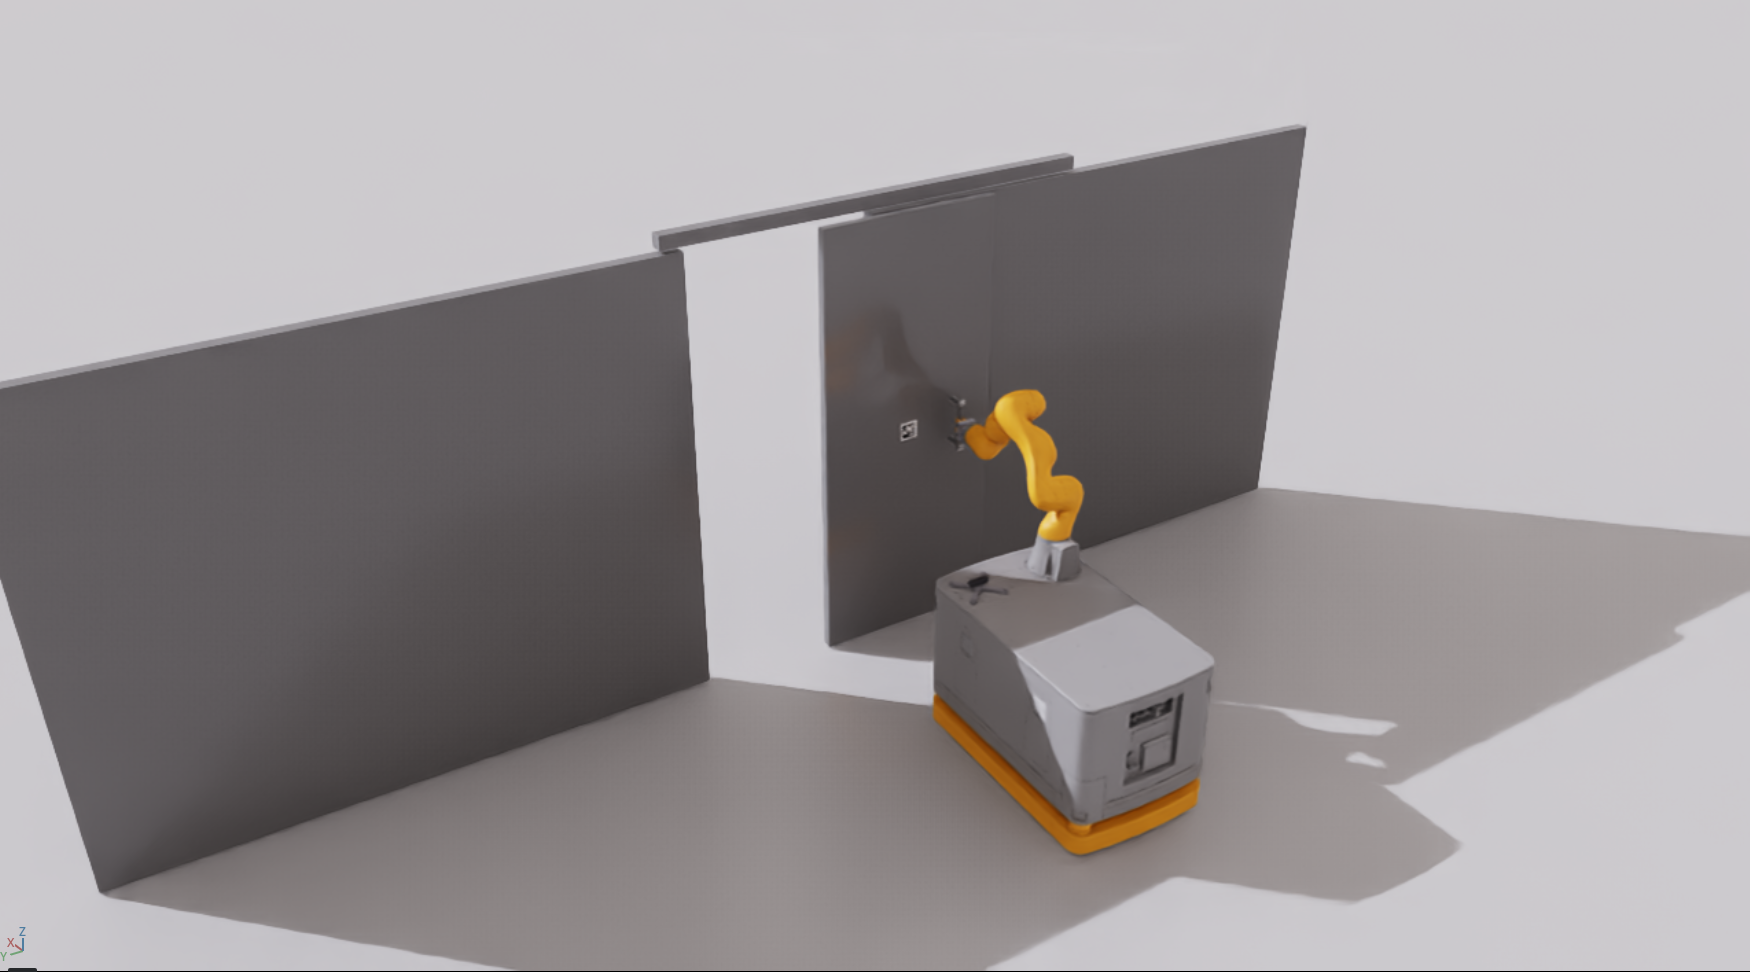
\includegraphics[width=\textwidth]{figures/kl_slike/kl_sliding_otvaranje.png}
            \caption{otvaranje}
      \end{subfigure}

      \vspace{4pt}
      \begin{subfigure}[b]{0.48\textwidth}
            \centering
            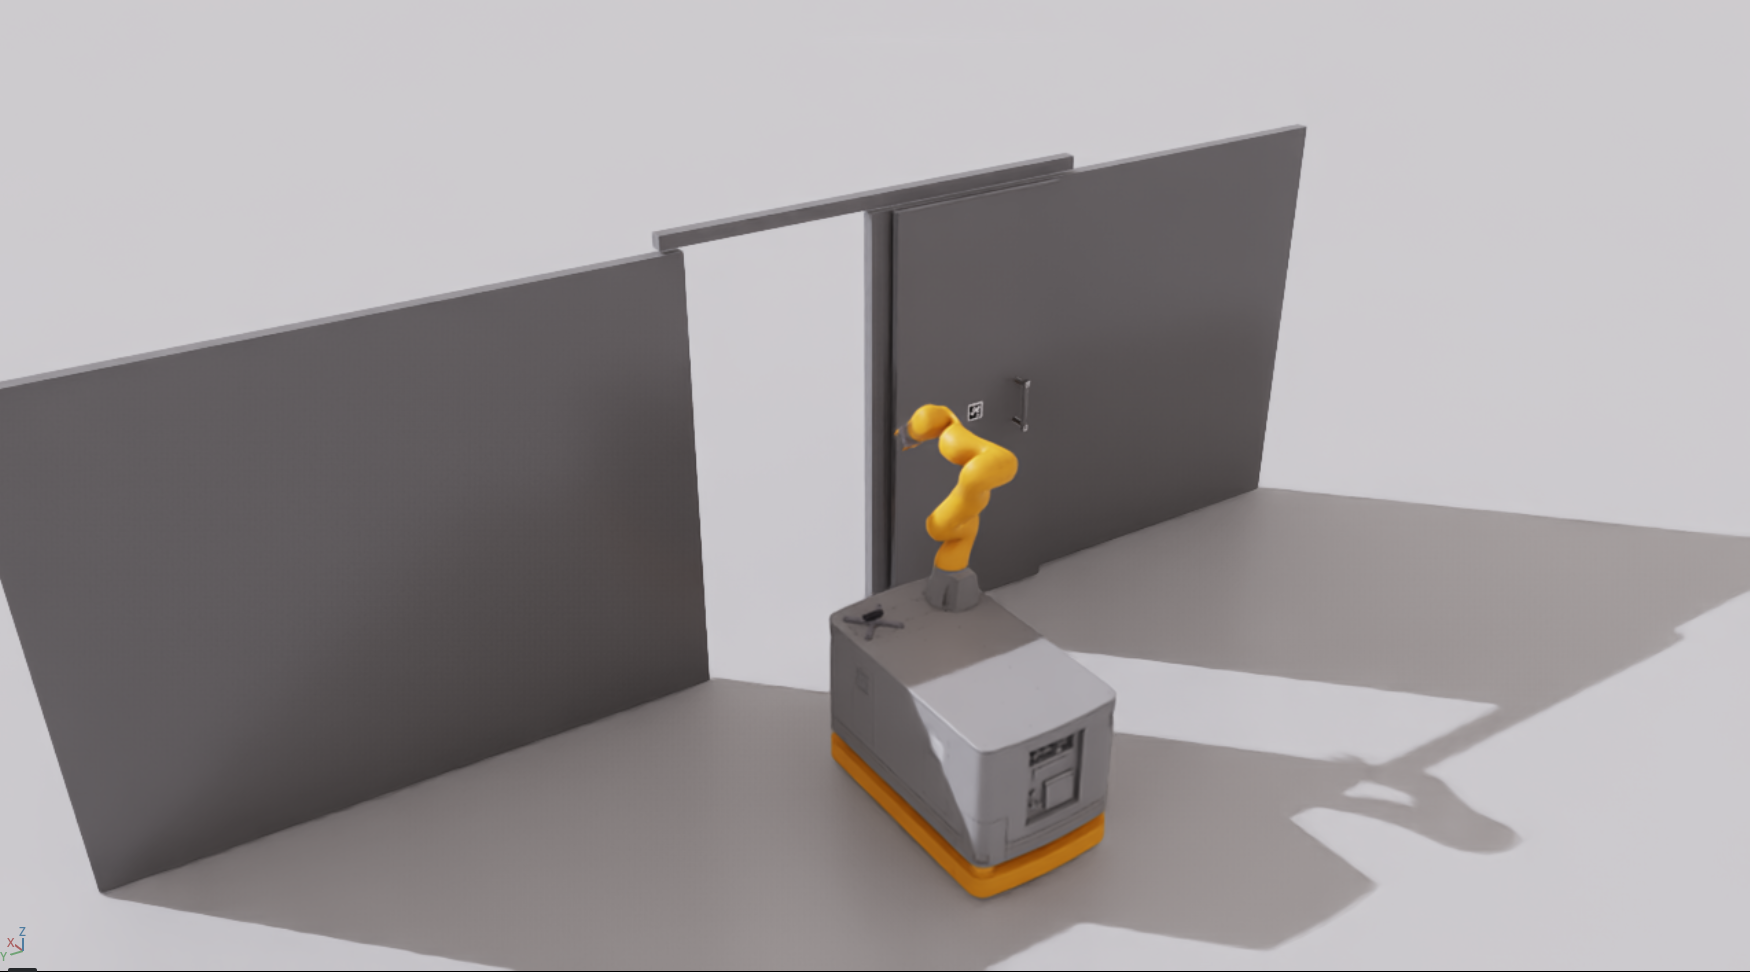
\includegraphics[width=\textwidth]{figures/kl_slike/kl_sliding_namjestanje.png}
            \caption{namještanje pred otvorom}
      \end{subfigure}
      \hfill
      \begin{subfigure}[b]{0.48\textwidth}
            \centering
            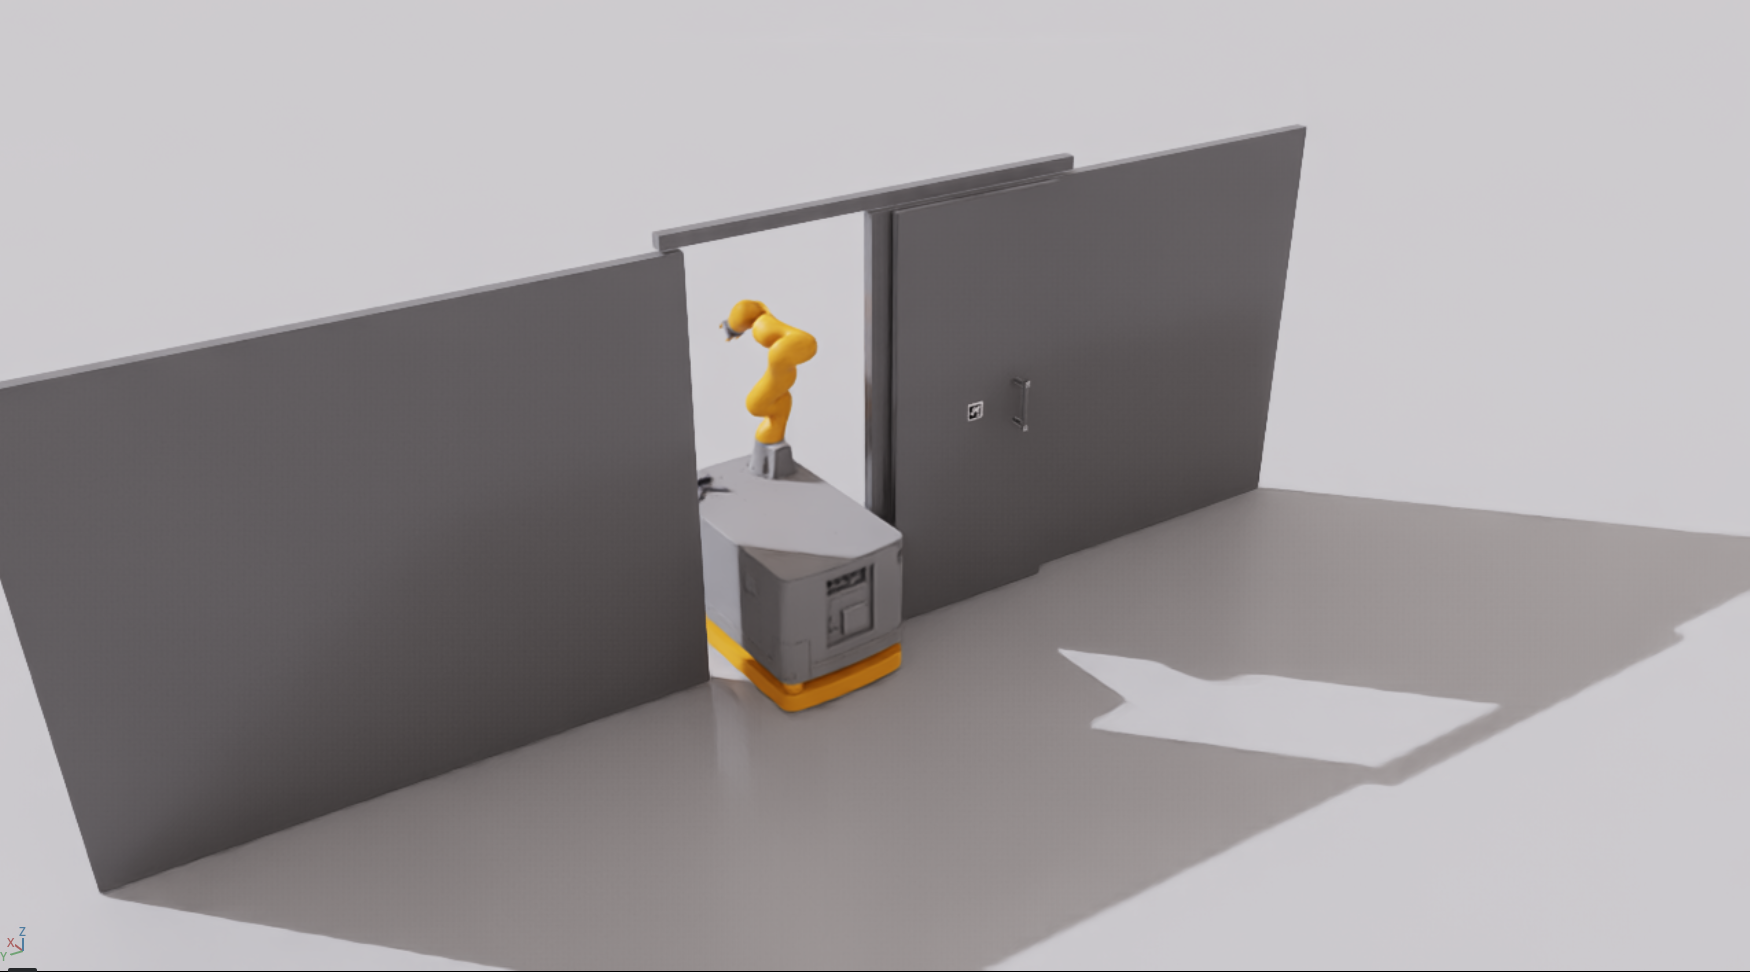
\includegraphics[width=\textwidth]{figures/kl_slike/kl_sliding_prolaz.png}
            \caption{prolazak kroz vrata}
      \end{subfigure}
      \caption{Faze izvođenja klasičnog pristupa na kliznim vratima}
      \label{fig:faze-klasicni-klizna}
\end{figure}

\subsection{Prilazak i hvat}

Pogreška poravnanja platforme iznosi 1,2 do 1,5\textdegree{}. Odstupanje postignute pred-hvatne poze od cilja
iznosi 8 do 11 mm u položaju te 0.1 do 0.2\textdegree{} u orijentaciji, a odstupanje same poze hvata 6 do
8 mm i oko 0.5\textdegree{}. Prepoznavanje tipa kvake iz geometrije (potpoglavlje \ref{sec:tip-kvake})
pokazalo se pouzdanim na objema scenama vrata.

\subsection{Zakretna vrata}

Guranje se zaustavlja na 70\textdegree{}, a završni zakret platforme
(potpoglavlje \ref{sec:zavrsni-zakret}) vrata doguruje do otprilike 100\textdegree{}, što je
dovoljno za prolazak. Izmjerene vrijednosti navedene su u tablici \ref{tab:rezultati-zakretna}.

\begin{table}[H]
      \centering
      \caption{Izmjerene vrijednosti pri otvaranju zakretnih vrata}
      \label{tab:rezultati-zakretna}
      \begin{tabular}{@{}ll@{}}
            \toprule
            Veličina                    & Vrijednost                                          \\
            \midrule
            Kut otvaranja guranjem      & 70\textdegree{} (cilj), 71\textdegree{}     stvarno \\
            Kut nakon završnog zakreta  & oko 100\textdegree{}                                \\
            Sila u hvatu, prosječna     & 320--450 N                                          \\
            Sila u hvatu, najveća       & do 630 N                                            \\
            Radijalno klizanje hvata    & do 8 mm                                             \\
            Pogreška praćenja položaja  & 0,4--2,5 mm                                         \\
            Pogreška procjene osi šarke & 5,8 mm prosječno, do 14,3 mm \ref{sec:provjera}     \\
            \bottomrule
      \end{tabular}
\end{table}

\subsection{Klizna vrata}

Ostvareno je otvaranje od 904 do 910 mm uz cilj od 900 mm, u dva prolaza, nakon čega je prolazak
kroz otvor uspješan. Sila u hvatu iznosila je u prosjeku 240 do 260 N, s vrhom do 660 N, a
klizanje hvata ostalo je između 4 i 6 mm kroz cijeli manevar. To je manje nego kod zakretnih
vrata, u skladu s time da se kod kliznih vrata smjer sile poklapa sa smjerom gibanja hvata, dok
kod zakretnih hvat prati zakrivljenu putanju. Prijeđeni put platforme iznosio je 900 mm, mjereno
odometrijom.

\section{Ograničenja}
\label{sec:klasicni-limits}

\begin{itemize}
      \item Gibanje platforme ima izraženu mrtvu zonu i ne postiže naređenu brzinu. Rotacija se
            ne pokreće ispod 0,36 rad/s, bočna translacija ispod otprilike 0,18 m/s, a uzdužna
            translacija postiže oko 45 \% naređenoga. Omjer je dosljedan kroz ispitani raspon
            brzina od 0,05 do 0,22 m/s, a brzina očitana u samom simulatoru odgovara naređenoj, pa
            je uzrok negdje u prijenosu naredbe do fizike platforme. Provjereno je i isključeno
            više mogućih uzroka: pogon i trenje u zglobu vrata, viskozno prigušenje platforme,
            brzina same simulacije te trajanje prijelazne faze na početku gibanja.
            Posljedica je da regulator koji zadaje male korekcije postaje dvopoložajan, jer je
            naredba ili ispod praga i bez učinka, ili puna.

      \item Prijeđeni put platforme ne smije se računati iz naređene brzine i vremena, iz
            prethodno navedenog razloga. Umjesto toga se mjeri odometrijom (potpoglavlje
            \ref{sec:odometrija}), pa se svi iznosi pomaka u ovom poglavlju odnose na izmjerenu,
            a ne na zadanu veličinu.

      \item Kako je navedeno u potpoglavlju \ref{sec:vrata}, zglob koji bi omogućio zakretanje
            kvake u konačnom je modelu nepomičan. Ta je odluka svjesno smanjenje opsega rada, ne
            nedostatak: zakretanje kvake bilo je u ranijoj fazi razvoja najproblematičniji dio
            zadatka, jer je kruto pozicijsko upravljanje tim dodatnim stupnjem slobode davalo
            velike kontaktne sile na svako odstupanje procjene. Uklanjanjem tog stupnja slobode
            zadatak je sveden na jedan stupanj slobode po tipu vrata. Ista je odluka primijenjena
            i u pristupu temeljenom na učenju, opisanom u poglavlju \ref{ch:rl}, čime ostaje
            osnova za usporedbu dvaju pristupa.

      \item Guranje zakretnih vrata ne prelazi otprilike 71\textdegree{}. Kako se vrata otvaraju,
            potreban doseg manipulatora raste s 0,81 na 0,88 m, a to se ne može nadoknaditi
            zakretanjem platforme, jer rotacija ima mrtvu zonu opisanu gore: svaki zakret kreće s
            barem 20\textdegree{}/s i slomi vezu između manipulatora i kvake. Ograničenje je
            zaobiđeno završnim zakretom platforme (potpoglavlje \ref{sec:zavrsni-zakret}),
            koji vrata doguruje do otprilike 100\textdegree{} bez opterećenja hvata.
            Otvaranje preko 100\textdegree{} zahtijevalo bi prepozicioniranje hvata, dakle
            puštanje kvake, premještanje platforme i ponovni hvat iz povoljnije konfiguracije, što
            nije izvedeno u opsegu ovog rada.

      \item Sustav sadrži zaseban postupak procjene geometrije ograničenja iz odnosa sile i
            gibanja, opisan u poglavlju \ref{ch:procjena}, ali on u klasičnom pristupu nije
            povezan s izvođenjem: os šarke u fazi otvaranja izračunava se geometrijski iz
            percepcije, a procjena iz gibanja postoji u zasebnim, samostalno pokretanim
            skriptama, izvan glavnog tijeka zadatka. Sustav zna i procijeniti ograničenje iz
            gibanja i otvoriti vrata, ali te dvije sposobnosti nisu spojene u jedan tijek
            izvođenja.

      \item Lidar tijekom otvaranja i prolaska prati postoji li prepreka neposredno ispred
            platforme i zaustavlja zadatak ako je udaljenost premala, ali ne raspolaže
            planiranjem puta niti izbjegavanjem prepreke.
\end{itemize}